\chapter{Một số lớp lỗ hổng bảo mật trên ứng dụng web}
% TODO: mô tả thêm những hướng có thể dựa trên background ở trên nhưng chỉ tập trung vào application layer và HTTP request/response
Trong phạm vi hiện thực công cụ, tôi chỉ tập trung vào việc tìm hiểu và phát hiện hai lỗ hổng bảo mật ở tầng ứng dụng của ứng dụng web, \acrfull{lfi} và time-based \acrlong{sqli} (SQLI). Đầu tiên, tôi sẽ trình bày về \acrfull{lfi}, một trong những lỗ hổng bảo mật phổ biến nhất trên ứng dụng web, luôn góp mặt trong top 10 lỗ hổng nguy hiểm nhất theo OWASP \parencite{owasp-top-10} nhiều năm gần đây. Nội dung phần này bao gồm làm rõ khái niệm \acrshort{lfi} và phân tích các kĩ thuật khai thác lỗ hổng bảo mật này.
\section{Local File Inclusion}
% https://www.rcesecurity.com/2017/08/from-lfi-to-rce-via-php-sessions/?fbclid=IwAR1VcA--iI7uRzwcqGk9JdcgHFZugVVNA1X2bLTSahRMhJy8Dk69gflKi8k
% https://outpost24.com/blog/from-local-file-inclusion-to-remote-code-execution-part-1
Lỗ hổng \acrfull{lfi} \parencite{portswigger-directory-traversal, sullivan2011web}, còn có tên khác là Directory Traversal, là lỗ hổng bảo mật trên ứng dụng web cho phép tin tặc đọc bất kì tập tin nào trên máy chủ mà ứng dụng web đang chạy trên. Những tập tin này có thể là mã nguồn, hình ảnh, dữ liệu hoặc thậm chí cả những tập tin hệ thống nhạy cảm. Trong một vài trường hợp xử lí phân quyền không tốt ở phía máy chủ, tin tặc còn có thể tạo thêm tập tin mới gây nên sự thay đổi dữ liệu và hành vi của ứng dụng, hoặc hắn có thể thực thi mã (\acrshort{rce}) từ phía máy chủ để chiếm quyền điều khiển hệ thống. Đoạn mã \ref{lst:php-lfi} dưới đây mô tả một điểm cuối của trang web ``\texttt{http://vuln-web.com/}'' có lỗ hổng \acrshort{lfi}.
\begin{lstlisting}[language=php, label={lst:php-lfi},caption={Đoạn mã PHP có lỗ hổng Local File Inclusion}]
/**
* Get the filename from a GET input
* Example - http://vuln-web.com/?file=filename.php
*/
$file = $_GET['file'];

/**
* Unsafely including the file
* Example - filename.php
*/
include('directory/' . $file);
\end{lstlisting}
Bằng cách nhận vào tham số \texttt{\$file} từ đường dẫn \acrshort{url}, máy chủ web trực tiếp trả về nội dung tập tin có tên \texttt{filename.php} trong thư mục hiện tại như trong ví dụ trên. Tin tặc có thể lợi dụng sơ hở từ câu lệnh \texttt{include('directory/' . \$file);} để trực tiếp đọc bất kì tập tin nào bằng cách sử đường dẫn tương đối, kết hợp tiền tố ``../'' (hoặc ``..\textbackslash'' đối với các máy chủ web dùng hệ điều hành Windows Server) để tham chiếu tới thư mục cha của thư mục hiện tại cộng với tên tập tin để đọc nội dung của tập tin đó, ví dụ như ``\texttt{http://vuln-web.com/?file=../../etc/passwd}''. Hình \ref{fig:lfi-payloads} sau đây minh họa một số vector tấn công (payload) dùng để đọc tập tin ``\textbf{passwd}'' trong đường dẫn \textbf{/etc/} trong các máy chủ web Unix.
\begin{figure}[H]
  \centering
    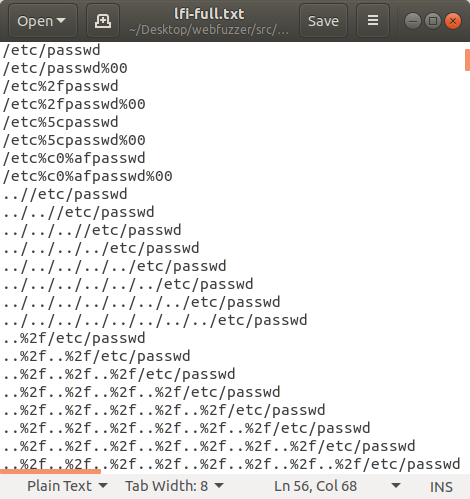
\includegraphics[width=0.7\textwidth,keepaspectratio=true]{images/lfi-payloads.png}
  \caption{Một số payload khai thác lỗ hổng \acrshort{lfi}}
  \label{fig:lfi-payloads}
\end{figure}
\textbf{/etc/passwd} là tập tin chứa danh sách tài khoản người dùng trên máy chủ web dùng hệ điều hành Unix, tập tin này bắt đầu bằng chuỗi ``\texttt{root:x}'' và chứa nhiều thông tin quan trọng như tên, địa chỉ email, đường dẫn tuyệt đối đến thư mục home trên đĩa cứng, ID của quyền (hoặc nhóm quyền) của người dùng đó,..., cung cấp cho tin tặc nhiều thông tin quý giá khi bắt đầu xâm nhập vào hệ thống. Do ta không biết độ sâu của thư mục ứng dụng web so với đường dẫn gốc (root directory) của hệ điều hành nên ta phải thử truy vấn đến từng tầng thư mục cha của thư mục hiện hành đến khi chạm tới thư mục gốc sau đó truy cập đến tập tin \textbf{/etc/passwd} như ví dụ trong Hình \ref{fig:lfi-payloads}.
\section{Time-based Structured Query Language Injection}
Hầu hết các kĩ thuật tấn công ứng dụng web đều tuân theo mô-típ đánh lừa ứng dụng web để thực hiện những hành động nguy hiểm thay tin tặc. Tin tặc không thể lấy được cookies của người dùng một cách chính quy nhưng có thể đánh lừa để trình duyệt web nạn nhân cung cấp cho hắn thông qua lỗ hổng \acrlong{xss} (\acrshort{xss}). Tin tặc cũng không thể tùy tiện truy xuất bất cứ tập tin nào trên máy chủ web nhưng hắn có thể lừa ứng dụng web làm việc đó thông qua lỗ hổng \acrshort{lfi}. Tương tự, tin tặc không thể trực tiếp truy cập và trích xuất cơ sở dữ liệu của ứng dụng web nhưng hắn có thể lừa ứng dụng web làm việc đó thông qua lỗ hổng \acrfull{sqli}. Phần này trình bày về khái niệm lỗ hổng \acrshort{sqli} nói chung và time-based \acrshort{sqli} nói riêng.\par
Lỗ hổng \acrfull{sqli} \parencite{li2011survey,sullivan2011web} cho phép tin tặc can thiệp vào các câu truy vấn \acrshort{sql} mà ứng dụng web dùng để tương tác với cơ sở dữ liệu. Thông thường việc này sẽ cho phép tin tặc đọc những dữ liệu mà hắn không có quyền, ví dụ như dữ liệu của những người dùng khác trong ứng dụng hoặc kể cả những dữ liệu mà ứng dụng đó không có quyền truy cập. Trong nhiều trường hợp tin tặc còn có thể sửa đổi hoặc sao chép (dump) những dữ liệu này, gây nên rủi ro bị đánh cắp dữ liệu và những hậu quả lâu dài cho nhà cung cấp ứng dụng web. Trong một vài điều kiện đặc biệt hơn, tin tặc còn có thể leo thang một cuộc tấn công \acrshort{sqli} để thỏa hiệp máy chủ ứng dụng web đang vận hành hoặc thực hiện một cuộc tấn công từ chối dịch vụ (\acrshort{dos} - \acrlong{dos}). Đoạn mã \ref{lst:php-sqli} sau đây là một ví dụ.
\begin{lstlisting}[language=php, label={lst:php-sqli},caption={Đoạn mã PHP\footnote{Nguồn: http://websec.fr/level01/source.php} có lỗ hổng SQL Injection}]
public function doQuery($injection) {
    $pdo = new SQLite3('database.db', SQLITE3_OPEN_READONLY);
    
    $query = 'SELECT id,username FROM users WHERE id=' . $injection . ' LIMIT 1';
    $getUsers = $pdo->query($query);
    $users = $getUsers->fetchArray(SQLITE3_ASSOC);

    if ($users) {
        return $users;
    }

    return false;
}
\end{lstlisting}
Câu truy vấn \acrshort{sql} trong ví dụ trên sẽ trả về cho người dùng giá trị của hai trường \texttt{id} và \texttt{username} của bản ghi đầu tiền trong bảng \texttt{users} có trường \texttt{id} bằng giá trị của tham số \texttt{\$injection} được truyền vào. Thông thường giá trị này thường là những chuỗi hoặc những con số có định dạng cụ thể, phục vụ cho việc truy vấn thông tin người dùng. Thông qua giao diện web hoặc \acrshort{http} request, tin tặc có thể can thiệp vào ứng dụng web và chỉnh sửa tùy ý nội dung của tham số \texttt{\$injection}. Ví dụ trong trường hợp giá trị tham số này là ``\colorbox{gray!30}{\texttt{1'; DROP TABLE users; -{}-'}}'', câu truy vấn trở thành\\
\colorbox{gray!30}{\texttt{SELECT id,username FROM users WHERE id='1'; DROP TABLE users; -{}-'}}\\
Sau khi truy vấn giá trị \texttt{id} và \texttt{username} của bản ghi có trường \texttt{id = 1} thì câu truy vấn \acrshort{sql} trên sẽ xóa toàn bộ nội dung (drop) bảng \text{users} trong cơ sở dữ liệu của ứng dụng. Bằng cách  thực hiện nhiều câu truy vấn nối tiếp hoặc lồng nhau (nested queries), đóng mở nháy đơn, sử dụng chú thích (-{}-) phù hợp với mã nguồn của trang web mà tin tặc có thể khai thác lỗ hổng \acrshort{sqli} này và gây ra hậu quả to lớn như thay đổi cấu trúc lược đồ quan hệ như ví dụ trên.\par
Lớp lỗ hổng \acrshort{sqli} có nhiều loại được phân ra dựa trên cách thức và mục tiêu tấn công \parencite{sqli-classification}, trong phạm vi luận văn này, tôi chỉ tập trung phát hiện lỗ hổng time-based \acrshort{sqli}. Time-based \acrshort{sqli} là kĩ thuật khai thác lỗ hổng \acrshort{sqli} bằng cách sử dụng những câu truy vấn đặc biệt, buộc hệ quản trị cơ sở dữ liệu phải chờ một khoảng thời gian trước khi trả về kết quả truy vấn cho ứng dụng, dựa vào thời gian phản hồi của câu truy vấn, ta có thể nhận định sự tồn tại của lỗ hổng này. Mục đích của việc kiểm thử lỗ hổng này không chỉ có vậy, việc khai thác thành công time-based \acrshort{sqli} trên những điểm cuối của một ứng dụng web còn có nghĩa là điểm cuối này cho phép truy vấn liên tiếp, lồng nhau, hoặc phát hiện được một số phần tử trong danh sách đen cũng như danh sách trắng của bộ lọc dữ liệu đầu vào, những nhận định này là cơ sở để tấn công sâu hơn vào ứng dụng web đó. Việc khai thác bằng kĩ thuật này phụ thuộc các hàm hoãn thời gian của mỗi hệ quản trị cơ sở dữ liệu khác nhau, cụ thể đối với MySQL ta dựa vào hàm \texttt{sleep} và \texttt{benchmark}, đối với Microsoft SQL Server là hàm \texttt{waitfor delay} và \texttt{waitfor time}, đối với Postgres SQL là \texttt{pg\_sleep},...
